\documentclass[twoside]{book}

% Packages required by doxygen
\usepackage{fixltx2e}
\usepackage{calc}
\usepackage{doxygen}
\usepackage[export]{adjustbox} % also loads graphicx
\usepackage{graphicx}
\usepackage[utf8]{inputenc}
\usepackage{makeidx}
\usepackage{multicol}
\usepackage{multirow}
\PassOptionsToPackage{warn}{textcomp}
\usepackage{textcomp}
\usepackage[nointegrals]{wasysym}
\usepackage[table]{xcolor}

% Font selection
\usepackage[T1]{fontenc}
\usepackage[scaled=.90]{helvet}
\usepackage{courier}
\usepackage{amssymb}
\usepackage{sectsty}
\renewcommand{\familydefault}{\sfdefault}
\allsectionsfont{%
  \fontseries{bc}\selectfont%
  \color{darkgray}%
}
\renewcommand{\DoxyLabelFont}{%
  \fontseries{bc}\selectfont%
  \color{darkgray}%
}
\newcommand{\+}{\discretionary{\mbox{\scriptsize$\hookleftarrow$}}{}{}}

% Page & text layout
\usepackage{geometry}
\geometry{%
  a4paper,%
  top=2.5cm,%
  bottom=2.5cm,%
  left=2.5cm,%
  right=2.5cm%
}
\tolerance=750
\hfuzz=15pt
\hbadness=750
\setlength{\emergencystretch}{15pt}
\setlength{\parindent}{0cm}
\setlength{\parskip}{3ex plus 2ex minus 2ex}
\makeatletter
\renewcommand{\paragraph}{%
  \@startsection{paragraph}{4}{0ex}{-1.0ex}{1.0ex}{%
    \normalfont\normalsize\bfseries\SS@parafont%
  }%
}
\renewcommand{\subparagraph}{%
  \@startsection{subparagraph}{5}{0ex}{-1.0ex}{1.0ex}{%
    \normalfont\normalsize\bfseries\SS@subparafont%
  }%
}
\makeatother

% Headers & footers
\usepackage{fancyhdr}
\pagestyle{fancyplain}
\fancyhead[LE]{\fancyplain{}{\bfseries\thepage}}
\fancyhead[CE]{\fancyplain{}{}}
\fancyhead[RE]{\fancyplain{}{\bfseries\leftmark}}
\fancyhead[LO]{\fancyplain{}{\bfseries\rightmark}}
\fancyhead[CO]{\fancyplain{}{}}
\fancyhead[RO]{\fancyplain{}{\bfseries\thepage}}
\fancyfoot[LE]{\fancyplain{}{}}
\fancyfoot[CE]{\fancyplain{}{}}
\fancyfoot[RE]{\fancyplain{}{\bfseries\scriptsize Generated by Doxygen }}
\fancyfoot[LO]{\fancyplain{}{\bfseries\scriptsize Generated by Doxygen }}
\fancyfoot[CO]{\fancyplain{}{}}
\fancyfoot[RO]{\fancyplain{}{}}
\renewcommand{\footrulewidth}{0.4pt}
\renewcommand{\chaptermark}[1]{%
  \markboth{#1}{}%
}
\renewcommand{\sectionmark}[1]{%
  \markright{\thesection\ #1}%
}

% Indices & bibliography
\usepackage{natbib}
\usepackage[titles]{tocloft}
\setcounter{tocdepth}{3}
\setcounter{secnumdepth}{5}
\makeindex

% Hyperlinks (required, but should be loaded last)
\usepackage{ifpdf}
\ifpdf
  \usepackage[pdftex,pagebackref=true]{hyperref}
\else
  \usepackage[ps2pdf,pagebackref=true]{hyperref}
\fi
\hypersetup{%
  colorlinks=true,%
  linkcolor=blue,%
  citecolor=blue,%
  unicode%
}

% Custom commands
\newcommand{\clearemptydoublepage}{%
  \newpage{\pagestyle{empty}\cleardoublepage}%
}

\usepackage{caption}
\captionsetup{labelsep=space,justification=centering,font={bf},singlelinecheck=off,skip=4pt,position=top}

%===== C O N T E N T S =====

\begin{document}

% Titlepage & ToC
\hypersetup{pageanchor=false,
             bookmarksnumbered=true,
             pdfencoding=unicode
            }
\pagenumbering{roman}
\begin{titlepage}
\vspace*{7cm}
\begin{center}%
{\Large My Project }\\
\vspace*{1cm}
{\large Generated by Doxygen 1.8.11}\\
\end{center}
\end{titlepage}
\clearemptydoublepage
\tableofcontents
\clearemptydoublepage
\pagenumbering{arabic}
\hypersetup{pageanchor=true}

%--- Begin generated contents ---
\chapter{Hierarchical Index}
\section{Class Hierarchy}
This inheritance list is sorted roughly, but not completely, alphabetically\+:\begin{DoxyCompactList}
\item \contentsline{section}{main\+\_\+savitch\+\_\+14\+:\+:game}{\pageref{classmain__savitch__14_1_1game}}{}
\begin{DoxyCompactList}
\item \contentsline{section}{main\+\_\+savitch\+\_\+14\+:\+:Mancala}{\pageref{classmain__savitch__14_1_1Mancala}}{}
\end{DoxyCompactList}
\end{DoxyCompactList}

\chapter{Class Index}
\section{Class List}
Here are the classes, structs, unions and interfaces with brief descriptions\+:\begin{DoxyCompactList}
\item\contentsline{section}{\hyperlink{classmain__savitch__14_1_1game}{main\+\_\+savitch\+\_\+14\+::game} }{\pageref{classmain__savitch__14_1_1game}}{}
\item\contentsline{section}{\hyperlink{classmain__savitch__14_1_1Mancala}{main\+\_\+savitch\+\_\+14\+::\+Mancala} }{\pageref{classmain__savitch__14_1_1Mancala}}{}
\end{DoxyCompactList}

\chapter{Class Documentation}
\hypertarget{classmain__savitch__14_1_1game}{}\section{main\+\_\+savitch\+\_\+14\+:\+:game Class Reference}
\label{classmain__savitch__14_1_1game}\index{main\+\_\+savitch\+\_\+14\+::game@{main\+\_\+savitch\+\_\+14\+::game}}


Inheritance diagram for main\+\_\+savitch\+\_\+14\+:\+:game\+:
\nopagebreak
\begin{figure}[H]
\begin{center}
\leavevmode
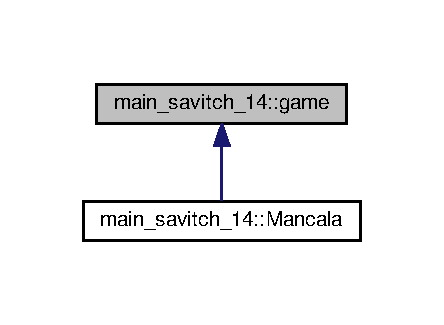
\includegraphics[width=213pt]{classmain__savitch__14_1_1game__inherit__graph}
\end{center}
\end{figure}
\subsection*{Public Types}
\begin{DoxyCompactItemize}
\item 
enum {\bfseries who} \{ {\bfseries H\+U\+M\+AN}, 
{\bfseries N\+E\+U\+T\+R\+AL}, 
{\bfseries C\+O\+M\+P\+U\+T\+ER}
 \}\hypertarget{classmain__savitch__14_1_1game_a4fe20fb287f809ae2b68e28e4ccba634}{}\label{classmain__savitch__14_1_1game_a4fe20fb287f809ae2b68e28e4ccba634}

\end{DoxyCompactItemize}
\subsection*{Public Member Functions}
\begin{DoxyCompactItemize}
\item 
who {\bfseries play} ()\hypertarget{classmain__savitch__14_1_1game_a4dbeaddb78059f7c5dcbf5cc4e026317}{}\label{classmain__savitch__14_1_1game_a4dbeaddb78059f7c5dcbf5cc4e026317}

\end{DoxyCompactItemize}
\subsection*{Protected Member Functions}
\begin{DoxyCompactItemize}
\item 
virtual void {\bfseries display\+\_\+message} (const std\+::string \&message) const \hypertarget{classmain__savitch__14_1_1game_ab8b87c3a1b68634861a8c0ed2b9f1992}{}\label{classmain__savitch__14_1_1game_ab8b87c3a1b68634861a8c0ed2b9f1992}

\item 
virtual std\+::string {\bfseries get\+\_\+user\+\_\+move} () const \hypertarget{classmain__savitch__14_1_1game_a1265f262f5a15bca5b532e6e97d13089}{}\label{classmain__savitch__14_1_1game_a1265f262f5a15bca5b532e6e97d13089}

\item 
virtual who {\bfseries last\+\_\+mover} () const \hypertarget{classmain__savitch__14_1_1game_a38d435da6aadc192ac10160b26ea0cc1}{}\label{classmain__savitch__14_1_1game_a38d435da6aadc192ac10160b26ea0cc1}

\item 
virtual int {\bfseries moves\+\_\+completed} () const \hypertarget{classmain__savitch__14_1_1game_aee677d1ef52c35474cb7c6071bb71749}{}\label{classmain__savitch__14_1_1game_aee677d1ef52c35474cb7c6071bb71749}

\item 
virtual who {\bfseries next\+\_\+mover} () const \hypertarget{classmain__savitch__14_1_1game_a0d445fdec3201c91c145ee2763e08922}{}\label{classmain__savitch__14_1_1game_a0d445fdec3201c91c145ee2763e08922}

\item 
virtual who {\bfseries opposite} (who player) const \hypertarget{classmain__savitch__14_1_1game_ae38d001e92ebe46e1a1433e41446c7ab}{}\label{classmain__savitch__14_1_1game_ae38d001e92ebe46e1a1433e41446c7ab}

\item 
virtual who {\bfseries winning} () const \hypertarget{classmain__savitch__14_1_1game_a081611c42aa66b4d91bbefeec47c7c4e}{}\label{classmain__savitch__14_1_1game_a081611c42aa66b4d91bbefeec47c7c4e}

\item 
virtual void {\bfseries make\+\_\+move} (const std\+::string \&move)\hypertarget{classmain__savitch__14_1_1game_a20597d0caa907aea47b27fed8be3759b}{}\label{classmain__savitch__14_1_1game_a20597d0caa907aea47b27fed8be3759b}

\item 
virtual void {\bfseries restart} ()\hypertarget{classmain__savitch__14_1_1game_ad521a7d78e7c163a0bc28b709f0d45fd}{}\label{classmain__savitch__14_1_1game_ad521a7d78e7c163a0bc28b709f0d45fd}

\item 
virtual \hyperlink{classmain__savitch__14_1_1game}{game} $\ast$ {\bfseries clone} () const =0\hypertarget{classmain__savitch__14_1_1game_a7b663057f59210dd52738facfc40d959}{}\label{classmain__savitch__14_1_1game_a7b663057f59210dd52738facfc40d959}

\item 
virtual void {\bfseries compute\+\_\+moves} (std\+::queue$<$ std\+::string $>$ \&moves) const =0\hypertarget{classmain__savitch__14_1_1game_a2c0c049f5861026d0f639b5837889b7a}{}\label{classmain__savitch__14_1_1game_a2c0c049f5861026d0f639b5837889b7a}

\item 
virtual void {\bfseries display\+\_\+status} () const =0\hypertarget{classmain__savitch__14_1_1game_ac8205178922c49bab2865187e834b726}{}\label{classmain__savitch__14_1_1game_ac8205178922c49bab2865187e834b726}

\item 
virtual int {\bfseries evaluate} () const =0\hypertarget{classmain__savitch__14_1_1game_a9b9c8c5e9aa57c9a430f20b87cb047aa}{}\label{classmain__savitch__14_1_1game_a9b9c8c5e9aa57c9a430f20b87cb047aa}

\item 
virtual bool {\bfseries is\+\_\+game\+\_\+over} () const =0\hypertarget{classmain__savitch__14_1_1game_a49eed20648918b03fd3e2cf78987b3d1}{}\label{classmain__savitch__14_1_1game_a49eed20648918b03fd3e2cf78987b3d1}

\item 
virtual bool {\bfseries is\+\_\+legal} (const std\+::string \&move) const =0\hypertarget{classmain__savitch__14_1_1game_ad38351422ca1ee3ae58440c1c6b36b30}{}\label{classmain__savitch__14_1_1game_ad38351422ca1ee3ae58440c1c6b36b30}

\end{DoxyCompactItemize}


The documentation for this class was generated from the following files\+:\begin{DoxyCompactItemize}
\item 
game.\+h\item 
game.\+cc\end{DoxyCompactItemize}

\hypertarget{classmain__savitch__14_1_1Mancala}{}\section{main\+\_\+savitch\+\_\+14\+:\+:Mancala Class Reference}
\label{classmain__savitch__14_1_1Mancala}\index{main\+\_\+savitch\+\_\+14\+::\+Mancala@{main\+\_\+savitch\+\_\+14\+::\+Mancala}}


Inheritance diagram for main\+\_\+savitch\+\_\+14\+:\+:Mancala\+:
\nopagebreak
\begin{figure}[H]
\begin{center}
\leavevmode
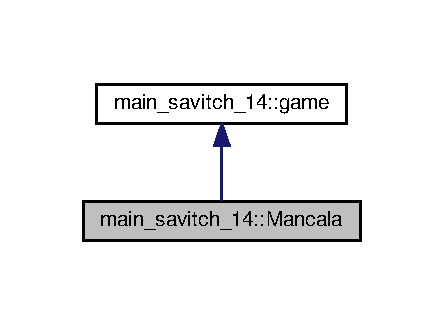
\includegraphics[width=213pt]{classmain__savitch__14_1_1Mancala__inherit__graph}
\end{center}
\end{figure}


Collaboration diagram for main\+\_\+savitch\+\_\+14\+:\+:Mancala\+:
\nopagebreak
\begin{figure}[H]
\begin{center}
\leavevmode
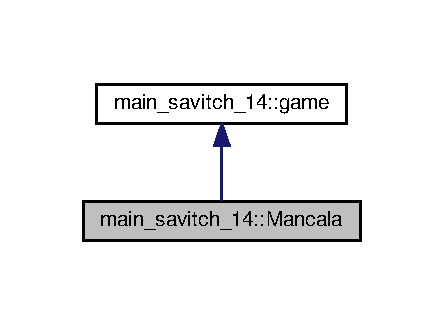
\includegraphics[width=213pt]{classmain__savitch__14_1_1Mancala__coll__graph}
\end{center}
\end{figure}
\subsection*{Public Member Functions}
\begin{DoxyCompactItemize}
\item 
void {\bfseries make\+\_\+move} (const std\+::string \&move)\hypertarget{classmain__savitch__14_1_1Mancala_a9cab7122179df32a128e1032d2071990}{}\label{classmain__savitch__14_1_1Mancala_a9cab7122179df32a128e1032d2071990}

\item 
void {\bfseries restart} ()\hypertarget{classmain__savitch__14_1_1Mancala_aeba0a1b17a315e1916197ca52a5a099b}{}\label{classmain__savitch__14_1_1Mancala_aeba0a1b17a315e1916197ca52a5a099b}

\item 
\hyperlink{classmain__savitch__14_1_1game}{game} $\ast$ {\bfseries clone} () const \hypertarget{classmain__savitch__14_1_1Mancala_a8158419b34c69ffc1fde1f58a82e8c31}{}\label{classmain__savitch__14_1_1Mancala_a8158419b34c69ffc1fde1f58a82e8c31}

\item 
void {\bfseries compute\+\_\+moves} (std\+::queue$<$ std\+::string $>$ \&moves) const \hypertarget{classmain__savitch__14_1_1Mancala_a5655c5e4494f3680007953ae58ecdc43}{}\label{classmain__savitch__14_1_1Mancala_a5655c5e4494f3680007953ae58ecdc43}

\item 
void {\bfseries display\+\_\+status} () const \hypertarget{classmain__savitch__14_1_1Mancala_a8e86ccccbe4cca4bcdcf5d08177785a0}{}\label{classmain__savitch__14_1_1Mancala_a8e86ccccbe4cca4bcdcf5d08177785a0}

\item 
int {\bfseries evaluate} () const \hypertarget{classmain__savitch__14_1_1Mancala_a1d7383671667bf085b98d3800b1c082f}{}\label{classmain__savitch__14_1_1Mancala_a1d7383671667bf085b98d3800b1c082f}

\item 
bool {\bfseries is\+\_\+game\+\_\+over} () const \hypertarget{classmain__savitch__14_1_1Mancala_aa12ed5d41262e363738e249ae8ad6132}{}\label{classmain__savitch__14_1_1Mancala_aa12ed5d41262e363738e249ae8ad6132}

\item 
bool {\bfseries is\+\_\+legal} (const std\+::string \&move) const \hypertarget{classmain__savitch__14_1_1Mancala_a8406fc376124313196bd531bd288b9eb}{}\label{classmain__savitch__14_1_1Mancala_a8406fc376124313196bd531bd288b9eb}

\end{DoxyCompactItemize}
\subsection*{Additional Inherited Members}


The documentation for this class was generated from the following files\+:\begin{DoxyCompactItemize}
\item 
mancala.\+h\item 
mancala.\+cc\end{DoxyCompactItemize}

%--- End generated contents ---

% Index
\backmatter
\newpage
\phantomsection
\clearemptydoublepage
\addcontentsline{toc}{chapter}{Index}
\printindex

\end{document}
